%\lstinputlisting[language=bash,basicstyle=\small]{python_codes/fieldstone_106/keywords.key}

\begin{center}
Code at \url{https://github.com/cedrict/fieldstone/tree/master/python_codes/fieldstone_106}
\end{center}

\par\noindent\rule{\textwidth}{0.4pt}

Last revision: September 17th, 2025.

\par\noindent\rule{\textwidth}{0.4pt}

%%%%%%%%%%%%%%%%%%%%%%%%%%%%%%%%%%%%%%%%%%%%%%%%%%%%%%%%%%%%%%%%%%%%%%%%%%%%%%%%%%%%%%%%%%%%%%%%%%%%

\Literature:\\
\fullcite{kiha92};\\
\fullcite{king97};\\
\fullcite{reki04};\\
\fullcite{kief03};\\
\fullcite{liki07};\\
\fullcite{legu12}.

\par\noindent\rule{\textwidth}{0.4pt}

\vspace{.5cm}

This stone is very much inspired by \textcite{keki97} (1997). 

\begin{center}
\includegraphics[width=6cm]{python_codes/fieldstone_106/images/keki97a}\\
{\captionfont Taken from \cite{keki97}.}
\end{center}

I set out to reproduce the results of the original publication. 
The necessary information for this exercise is spread out throughout the first pages
of the paper. In Section~3 it is stated that the angular opening is $\pi/4$ and $r_i/r_o=0.55$.
However, it is not clear what $r_i$ or $r_o$ are, although Section~3
mentions $r$ values of 1.7 which is somewhat in the 'middle' of the cone. 
Because the equations in the paper are in dimensionless form, and 
because it is common to choose the depth of the mantle as reference length, 
then we probably have $r_o-r_i=1$. In this case we find $r_i=1.22\dots$ and 
$r_o=2.22\dots$ ({\color{orange} 1st guess}: confirmed by author S.K., June 2021. 
Also consistent with \textcite{king97} (1997)).

Free-slip boundary conditions are imposed on all boundaries.
A patch on the inner boundary of the shell is heated by
maintaining it at a constant dimensionless temperature of $T_{patch}=1$; 
elsewhere the base of the shell is insulating ($\partial T/\partial r = 0$).
At the top of the shell, a constant dimensionless temperature of $T_{top}=0$ was maintained.
Unfortunately it is not specified how wide the patch is, so I choose 
$\pi/8$ which seems probable when looking at 
Figure~3 of the paper ({\color{orange} 2nd guess}: confirmed by S.K., June 2021).
The sides of the cone are insulating ($\partial T/\partial \theta =0$).
Because of how FE works the insulating boundary conditions are automatically enforced 
when Dirichlet boundary conditions are absent. 

The viscous rheology is temperature-dependent:
\[
\eta(T) =\eta_0 \exp\left[ E \left( \frac{1}{T+T_0} -\frac{1}{1+T_0}  \right)   \right]
\]
with $E= \{0,0.25328,3\}$. $T_0$ is defined as ``the surface temperature divided by the temperature
drop across the shell'' but its value is not specified. On Earth the surface temperature 
is $\sim300\si{\kelvin}$
while the temperature drop across the mantle is $\sim3000\si{\kelvin}$ 
so I take $T_0=0.1$ ({\color{orange} 3rd guess}: S.K. says that $\Delta T$ can be recovered from 
the Rayleigh number and using standard Earth values for all other parameters, but given the uncertainty about 
the Rayleigh number itself, this parameter is lost forever).
The value for $\eta_0$ is also not specified but if this value is used as reference viscosity value 
during the adimensionalisation process then $\eta_0=1$ ({\color{orange} 4th guess}).i
As indicated in the paper, the viscosity is ``clipped'' to $1000\eta_0$.
The initial temperature in the domain is set to $T=0.25$.

As seen in Section~\ref{MMM-ss:dimeqs2}, the dimensionless heat transport equation 
is void of any coefficient if $\kappa/h$ is used as a reference velocity 
(where $h$ is a reference length) so we take the 
dimensionless value of $\kappa$ to be 1 in Eq.~5 of the paper.   

Looking at Eq.~1 we find that there probably is a factor 2 missing before 
the viscosity $\mu$ ({\color{orange} 5th guess}: confirmed by S.K., June 2021).
In Section~2.2 it is stated that the SUPG method is used (see Section~\ref{MMM-ss:supg}) 
but how the stabilisation parameter
is chosen is not specified ({\color{orange} 6th guess}).

In the end the set of equations solved by the code is as follows:
\begin{eqnarray}
-\vec\nabla p + \vec\nabla \cdot(2 \eta \dot{\bm \varepsilon} ) &=& \Ranb \; T \vec{e}_r \\
\vec\nabla\cdot\vec\upnu &=& 0 \\
\frac{\partial T}{\partial t} + \vec\upnu\cdot\vec\nabla T &=& \Delta T 
\end{eqnarray}
Given the above boundary conditions, initial temperature and Rayleigh number value $\Ranb=10^7$ these
equations can be solved. 

Concerning the value of $\Ranb$, it is said to be $10^7$ but preliminary runs (in 2D) yield much 
narrower plumes for the isoviscous case than in the paper. However using $10^6$ 
instead seems to visually match the paper's results. I asked S.K. whether 
there could not be a mistake in the reported Ra in the paper and he kindly answered the following:
"A mistake is always possible. Here’s a possibility: the $\Ranb=10^7$ was what was input into the 
input file but we did not do a proper internal scaling to account for this, i.e. 
$r_o^3$ was used rather than $(r_o-r_i)^3$ with $r_o^3 = 2.22^3 \sim 10$.  
Usually in our codes what we put in as the Rayleigh number is really rho-g-alpha and all the other factors are 
input as 1 (or implicitly assumed to be 1).  
At any rate, I suspect $10^6$ could be a result of not accounting properly for the radius not being 1.0.  
I found some files one of my students used circa 2007 and the Ra was set to $10^7$ in the input file 
while the grid (different file) was $1.2 \rightarrow 2.2$.  I could see how one would forget 
when it comes to writing up the paper."

The paper mentions dimensioned quantities twice: in the caption of Fig.~3, we 
learn that 
$t=0.000561$ corresponds to $1.5\cdot 10^8\si{\year}$,
$t=0.000730$ corresponds to $2.0\cdot 10^8\si{\year}$, and
$t=0.016353$ corresponds to $4.4\cdot 10^9\si{\year}$.
This yields a reference time of about 270e9, which is close 
to  the one obtained as $t_{ref}=h^2/\kappa = 
(2891e3)^2/10^{-6}\sim 8.36\cdot 10^{18}s \sim 265\cdot 10^9 \si{\year}$
(see Section~\ref{MMM-ss:dimeqs2}).

This stone relies on $Q_2\times Q_1$ elements while the orginal paper relies
on the cheaper $Q_1\times P_0$ element with a penalty formulation (the 
value of the penalty parameter is also not mentioned). 

The user chooses the number of elements in the 
radial direction $nelr$ and the number of elements in the tangential direction is automatically 
computed as $nelt=1.5\cdot nelr$.
Elements on the boundaries are flagged by means of the $flag\_el\_X$ array ($X=1,2,3,4$ 
corresponding to left, right, bottom and top). 
Similar boolean arrays are setup for nodes on the boundaries: $flag\_X$. 
Free-slip boundary conditions are more difficult to impose than for Cartesian domains 
because the boundaries of the computational domain are either curved and/or not aligned
with the Cartesian axis. 
The timestep is computed by means of a CFL criterion, but it is limited to a $2\times$ 
increase from one time step to the next to insure a somewhat smooth transition at 
the beginning when the plume is rising faster and faster.
Because the lithostatic pressure does not contribute to the calculations and has effectively
been removed from the equations the pressure that is being solved for is the dynamic pressure. 
We can therefore run models with open boundary conditions on the side walls. This is 
controlled by the $use\_fs\_on\_sides$ parameter. If this parameter is true then there is a 
rotational nullspace and it is removed by setting $\vec\upnu=\vec{0}$ at $x=0$ and $y=r_i$.
This option was not explored in the original paper.

The equations are solved in their cylindrical axisymmetric form, see
Section~\ref{MMM-ss:axicyleqs}. Their FE discretisation is presented in Section~\ref{MMM-ss:cyl_axi}
and Section~\ref{MMM-ss:hte_axisym}.


\begin{remark}
LK filter and/or SUPG should be tested (at the moment the temperature us thresholded in the 
material model). Explore resolution, initial T in the mantle, try scaled-down Steinberger average 
viscosity profile, look at dynamic topography, strain-rate dependent power-law rheology, different 
Ra number, ... finish scaling up to real Earth like dimensions.
Would be nice to normalise the pressure on the top surface, not only a corner.
Also remove all bc on sides and use reduced density only? 
\end{remark}

%------------------------------------------------
\subsubsection*{Computing surface tractions}

Pressure normalised to be zero in the upper right corner so as to remove the nullspace. 
It is then projected onto the velocity nodes. This quantity is then normalised so that 
the average pressure at the surface is zero. 

Because of the axisymmetry the deviatoric stress tensor and stress tensor 
are given by
\[
{\bm \tau} 
= 
\left(
\begin{array}{ccc}
\tau_{rr} & \tau_{r\theta} & \tau_{rz} \\
\tau_{\theta r} & \tau_{\theta \theta} & \tau_{\theta z} \\
\tau_{zr} & \tau_{z\theta} & \tau_{zz} 
\end{array}
\right)
=
\left(
\begin{array}{ccc}
\tau_{rr} & 0 & \tau_{rz} \\
0  & \tau_{\theta \theta} & 0 \\
\tau_{zr} & 0 & \tau_{zz} 
\end{array}
\right)
\qquad
\text{and}
\qquad
{\bm \sigma} = -p {\bm 1} + {\bm \tau}
\]
The traction at the surface is given by 
\[
\vec{t}_n 
= {\bm \sigma}\cdot \vec{n}
=
\left(
\begin{array}{c}
\sigma_{rr} n_r + \sigma_{rz} n_z \\
0 \\
\sigma_{zr} n_r + \sigma_{zz} n_z
\end{array}
\right)
\]
and the normal component of the traction by 
\[
t_n= \vec{t}_n \cdot \vec{n} = \sigma_{rr} n_r^2 + 2 \sigma_{rz} n_r n_z + \sigma_{zz} n_z^2
\]




%%%%%%%%%%%%%%%%%%%%%%%%%%%%%%%%%%%%%%%%%%%%%%%%%%%
\subsubsection*{Scaling it back up}

What follows is an attempt at using the regular equations with Earth-like values for parameters...

As explained in Section~\ref{MMM-ss:dimeqs2} we choose four reference quantities:
\begin{itemize}
\item the reference length $L_{ref}=r_o-r_i=2891\si{\kilo\metre}$ (trivial choice)
with $r_i=3480\si{\km}$ and $r_o=6371\si{\km}$.


\item the reference temperature $T_{ref}=\Delta T = 3000\si{\kelvin}$ (trivial choice)

\item the thermal diffusion coefficient $\kappa_{ref}$. From Warren \etal \cite{wabj08}:
$\rho_0=3250\si{\kg\per\cubic\metre}$,  $k=2.25 \si{\watt\per\metre\per\kelvin}$,  $C_p=1250 \si{\joule\per\kelvin}$
so 
\[
\kappa = \frac{k}{\rho C_p} =	\frac{2.25}{3250 \cdot 1250} \simeq 5.5\cdot 10^{-7} 
\]
so we take $\kappa_{ref} = 5.5\cdot 10^{-7} \si{\square\metre\per\second}$.

\item the reference viscosity $\eta_{ref}$. The Rayleigh number is defined by
\[
\Ranb 
= \frac{\rho_0 g \alpha \Delta T (r_o-r_i)^3}{\eta_0 \kappa}
=\frac{\rho_0^2 C_p g \alpha \Delta T (r_o-r_i)^3}{\eta_0 k}
\]
with $\alpha=3\cdot 10^{-5} \si{\per\kelvin}$ and $g=9.81\si{\metre\per\square\second}$
so 
\[
\eta_{ref}=\eta_0 =\frac{\rho_0^2 C_p g \alpha \Delta T (R_{outer}-R_{inner})^3}{\Ranb \; k}
\simeq 1.25 \cdot 10^{22}\si{\pascal\second}
\]
which is a very acceptable value for the mantle viscosity, see Section~\ref{MMM-ss:viscprof}.
\end{itemize}

\noindent The dimensionless viscosity is either constant ($\eta_0'=1$) or temperature-dependent 
\[
\eta'(T')
=\eta_0' \exp\left[ \frac{E}{R \Delta T} \left( \frac{1}{T'+t_0} -\frac{1}{1+t_0}  \right)   \right]
%=\eta_0' \exp\left[ \frac{E}{R} \left( \frac{1}{T' \Delta T  +t_0 \Delta T} -\frac{1}{\Delta T +t_0 \Delta T}  \right)   \right]
\]
where ``$t_0$ is the surface temperature $T_{surf}$ divided by 
the temperature drop across the shell $\Delta T$''.
Assuming that the authors used 
\[
T'=\frac{T-T_{surf}}{T_{patch}-T_{surf}}= \frac{T-T_{surf}}{\Delta T}
\]
then (after multiplying the equation above by $\eta_{ref}$): 
\[
\eta(T)
=\eta_0 \exp\left[ \frac{E}{R} \left( \frac{1}{T-T_{surf}  + T_{surf}} 
-\frac{1}{T_{patch}-T_{surf} + T_{surf}}  \right)   \right]
=\eta_0 \exp\left[ \frac{E}{R} \left( \frac{1}{T} -\frac{1}{T_{patch}}\right) \right]
\]
so that $\eta(T_{patch})=\eta_0$. The authors investigate three cases:
\[
\frac{E}{R \Delta T} = \{0,0.25328,3\}
\]
With $R=8.31$ and $\Delta T=3000\si{\kelvin}$ then $E=\{ 0, 6317.6 , 74829.6 \}$ which 
are rather low values for an activation energy. 

Note that the rheology can be written:
\[
\eta(T)  
= \frac12 \underbrace{2 \eta_0  \exp\left( -\frac{E}{R T_{patch}} \right) }_{A^{-1}} \exp \frac{E}{R T}  
\]
which is effectively a diffusion creep type viscosity.
We find that for $T_{patch}=3000+273=3273$: 
\[
A^{-1} = \{ 2.5e22, 1.98e22 , 1.6e21 \}
\]
or, 
\[
A = \{ 4\cdot 10^{-24}    , 5.05\cdot 10^{-24}   ,  6.26\cdot 10^{-23}\} 
\]
From the four reference values above we can construct additional ones, 
such as the reference stress, which we will need to look at dynamic topography.
From Section~\ref{MMM-ss:dimeqs2}:
\[
\sigma_{ref} 
= \eta_{ref} \dot{\varepsilon}_{ref} 
= \eta_{ref} \frac{\kappa_{ref}}{L^2_{ref}} 
= \eta_0 \frac{\kappa }{ (r_o-r_i)^2}
= \frac{\rho_0 g \alpha \Delta T (r_o-r_i)^3}{\Ranb \; \kappa} \frac{\kappa}{(r_o-r_i)^2}
= \frac{\rho_0 g \alpha \Delta T (r_o-r_i)}{\Ranb}
\simeq 829.55  
\] 


Of course this exercise is somewhat silly as the values of most material parameters
vary with depth, temperature, etc ... and the choices I have made so far are rather arbitrary.

The following results obtained on various meshes. 
No SUPG. The CFL number is set to 1. 
$Q_2\times Q_1$ elements are used. 

\newpage
%%%%%%%%%%%%%%%%%%%%%%%%%%%%%%%%%%%%%%%%%%%%%%%%%%%
\subsubsection*{Isoviscous model - $Ra=10^6$}

\begin{center}
\includegraphics[width=15cm]{python_codes/fieldstone_106/images/keki97b}
\end{center}


\begin{center}
\includegraphics[width=5cm]{python_codes/fieldstone_106/results/axi/vrms1}
\includegraphics[width=5cm]{python_codes/fieldstone_106/results/axi/Tavrg1}
\includegraphics[width=5cm]{python_codes/fieldstone_106/results/axi/stats_T1}\\
\includegraphics[width=5cm]{python_codes/fieldstone_106/results/axi/profile_T1}
\includegraphics[width=5cm]{python_codes/fieldstone_106/results/axi/profile_eta1}
\end{center}




\newpage
%%%%%%%%%%%%%%%%%%%%%%%%%%%%%%%%%%%%%%%%%%%%%%%%%%%
\subsubsection*{Weakly temperature-dependent model - $Ra=10^6$}
\begin{center}
\includegraphics[width=15cm]{python_codes/fieldstone_106/images/keki97c}
\end{center}

\begin{center}
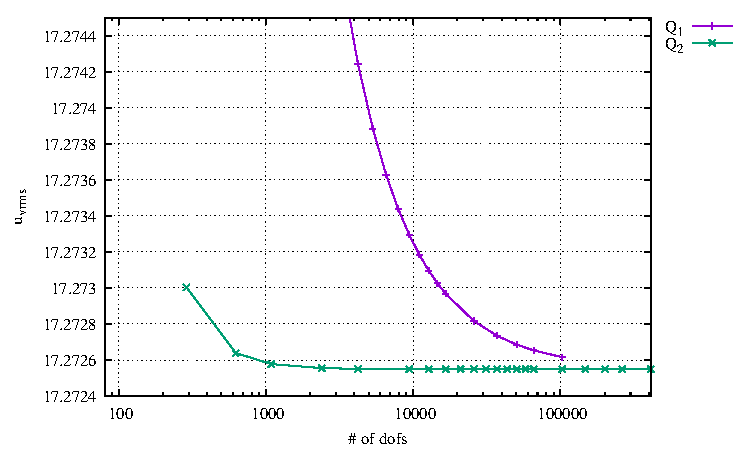
\includegraphics[width=5cm]{python_codes/fieldstone_106/results/axi/vrms2}
\includegraphics[width=5cm]{python_codes/fieldstone_106/results/axi/Tavrg2}
\includegraphics[width=5cm]{python_codes/fieldstone_106/results/axi/stats_T2}\\
\includegraphics[width=5cm]{python_codes/fieldstone_106/results/axi/profile_T2}
\includegraphics[width=5cm]{python_codes/fieldstone_106/results/axi/profile_eta2}
\end{center}




\newpage
%%%%%%%%%%%%%%%%%%%%%%%%%%%%%%%%%%%%%%%%%%%%%%%%%%%
\subsubsection*{Strongly temperature-dependent model - $\Ranb=10^6$}
\begin{center}
\includegraphics[width=15cm]{python_codes/fieldstone_106/images/keki97d}
\end{center}


\begin{center}
\includegraphics[width=5cm]{python_codes/fieldstone_106/results/axi/vrms3}
\includegraphics[width=5cm]{python_codes/fieldstone_106/results/axi/Tavrg3}
\includegraphics[width=5cm]{python_codes/fieldstone_106/results/axi/stats_T3}\\
\includegraphics[width=5cm]{python_codes/fieldstone_106/results/axi/profile_T3}
\includegraphics[width=5cm]{python_codes/fieldstone_106/results/axi/profile_eta3}
\end{center}


